\documentclass[sigconf,nonacm]{acmart}

\setcopyright{none}
\settopmatter{printacmref=true,printfolios=true}
\renewcommand\footnotetextcopyrightpermission[1]{}

\acmConference[ICCAD '26]{International Conference on Computer-Aided Design}{2026}{TBD}
\acmBooktitle{ICCAD '26: International Conference on Computer-Aided Design}
\acmDOI{}
\acmISBN{}

\usepackage{booktabs}
\usepackage{amsmath}
\usepackage{enumitem}
\usepackage{xspace}
\usepackage{multirow}
\usepackage{graphicx}
\usepackage{array}

\newcommand{\rsad}{R-SAD\xspace}
\newcommand{\sysmix}{SysMix\xspace}
\newcommand{\fmax}{F\textsubscript{max}\xspace}
\newcommand{\wns}{WNS\xspace}
\newcommand{\tns}{TNS\xspace}
\newcommand{\hpwl}{HPWL\xspace}

\title{Timing-Driven DSP Placement for Systolic Arrays on FPGAs}

\ccsdesc[500]{Hardware~Reconfigurable logic and FPGAs}
\keywords{FPGA placement, systolic arrays, DSP placement, timing-driven placement, dynamic programming}

\author{Anonymous Author(s)}
\affiliation{%
  \institution{Anonymous Institution}
  \city{Anonymous City}
  \country{Anonymous Country}
}
\email{anonymous@anonymous.edu}
\raggedbottom
\AtBeginDocument{\let\balance\relax}

\begin{document}

\begin{abstract}
Systolic-array-based field-programmable gate array (FPGA) accelerators exhibit strong spatial regularity, yet their timing quality remains highly sensitive to placement. Existing FPGA placers are largely general-purpose. Our previous \rsad-based flow identified an order-consistency (OC) structural viewpoint for systolic-array placement~\cite{rsad2023}. In this work, we develop a timing-driven digital signal processing (DSP) placement method that builds on this structural foundation. We first justify the use of OC from the half-perimeter wirelength (\hpwl) viewpoint, and then show that the resulting weighted multi-net placement objective can be reduced to a shortest-path problem on a state directed acyclic graph (DAG). This yields an exact dynamic-programming (DP) solver for the fixed-weight subproblem and enables iterative timing-driven reweighting. Averaged over seven benchmarks, the proposed flow improves maximum frequency (\fmax) by 7.4\% over Vivado and by 4.8\% over \rsad, while reducing \hpwl by 24.0\% relative to Vivado and incurring only a 1.9\% increase relative to \rsad. These results show that explicitly controlling the longest wirelength improves worst negative slack (\wns) and \fmax while preserving essentially the same \hpwl quality as the \hpwl-oriented predecessor.

\end{abstract}

\maketitle

% Target page allocation for the 8-page ICCAD draft:
% Introduction: 1.0--1.2 pages
% Background + formulation: 0.6--0.8 pages
% Method: 2.0--2.5 pages
% Experimental setup + results: 2.0--2.5 pages
% Related work + conclusion: 0.8--1.0 page

\section{Introduction}

Systolic arrays are a dominant compute substrate in machine-learning (ML) acceleration on field-programmable gate arrays (FPGAs). Their implementations are typically digital signal processing (DSP)-heavy and structurally regular. However, this regularity does not by itself guarantee good timing. Once mapped to a heterogeneous FPGA fabric, a systolic array is strongly affected by long inter-processing-element (PE) connections, so placement has a direct impact on worst negative slack (\wns) and maximum frequency (\fmax).

This setting exposes a clear mismatch between generic FPGA placement and systolic-array placement. General-purpose placers do not explicitly exploit the structural regularity of the array. Our previous work, centered on the \rsad algorithm, addressed this issue by introducing an order-consistency (OC) structural viewpoint for systolic-array placement and showing that this viewpoint can lead to strong half-perimeter wirelength (\hpwl) results~\cite{rsad2023}. The present work builds on that foundation. Its goal is not to replace \rsad as an \hpwl-oriented predecessor, but to extend the same structural line to the timing-driven setting.

The key difficulty is that timing-driven placement is not a single-metric \hpwl problem. On FPGAs, timing is strongly influenced by the longest critical wires, so improving \fmax requires more than reducing aggregate wirelength alone. The method therefore must optimize multiple nets under nonuniform timing-dependent weights while preserving the structural advantages identified by \rsad.

The main contribution of this paper is a formulation result. We first justify the OC condition from the \hpwl viewpoint, and then show that the resulting weighted multi-net objective can be reduced to the optimization of one shortest path on a state DAG. This converts the strip-placement problem into a dynamic-programming problem with exact optimal substructure for fixed weights. It also explains why the \rsad line is scientifically meaningful: once order consistency is justified, the single-column placement problem admits exact optimization rather than only heuristic search.

Based on this formulation, we build a timing-driven placement flow that iteratively adjusts net weights according to timing pressure and repeatedly invokes the DP solver. On the seven benchmarks in our current study, the resulting flow improves average \fmax by 7.4\% over Vivado and by 4.8\% over our previous \rsad-based method. At the same time, it reduces average \hpwl by 24.0\% relative to Vivado, while increasing \hpwl by only 1.9\% relative to \rsad. It also improves average \wns and total negative slack (\tns) over both baselines. These numbers support the central claim of this paper: explicitly controlling the longest wirelength is an effective path toward reducing \wns and improving \fmax for systolic-array DSP placement, while preserving nearly the same \hpwl quality as \rsad.

The contributions of this paper are summarized as follows.
\begin{itemize}[leftmargin=*,topsep=2pt,itemsep=2pt]
\item We further clarify the role of the OC condition introduced by \rsad and show how it turns the single-column DSP placement objective into an ordered form that is compatible with exact shortest-path optimization.
\item We formulate timing-driven DSP placement for systolic arrays on FPGAs through a weighted multi-net objective and show that it can be converted into the shortest-path optimization of a state DAG.
\item We develop a DP solver that is applicable to different net-weight settings, which makes it suitable for timing-driven reweighting rather than only one fixed deterministic placement policy.
\item We build a timing-driven placement flow that improves average \fmax by 7.4\% over Vivado and 4.8\% over the previous \rsad-based method, while reducing average \hpwl by 24.0\% versus Vivado and incurring only a 1.9\% \hpwl increase over \rsad.
\end{itemize}

The rest of the paper is organized as follows. Section~\ref{sec:rw} reviews the most relevant background. Section~\ref{sec:problem} introduces the problem setting and notation. Section~\ref{sec:method} presents the multi-column decomposition, the state-DAG formulation, and the timing-driven flow. Section~\ref{sec:exp} describes the experimental setup and results. Section~\ref{sec:conclusion} concludes the paper.

\section{Related Work}
\label{sec:rw}

\subsection{Systolic-Array-Specific Placement}

Our previous work on systolic-array placement on FPGAs established that exploiting array regularity can substantially improve placement quality over generic FPGA placement flows~\cite{rsad2023}. That work introduced the \rsad algorithm together with the order-consistency (OC) condition. OC is the most relevant predecessor idea for the present paper: it states that the spatial order of processing elements should follow their array order, thereby turning single-column placement into a structured ordered problem rather than an unconstrained generic placement problem. The \rsad line also motivates the region-wise decomposition used in this paper. In particular, for tall single-column strips, the central row-sweep (CTR) region serves as a structural pattern that can be exploited for acceleration by reducing an $m \times h$ problem to an $h \times h$ core problem before reconstruction.

More recently, \sysmix extended the same research line toward mixed-size placement for hierarchical systolic-array designs~\cite{sysmix2024}. The key message from these works is that systolic-array placement benefits from explicit structural modeling. However, they do not address the weighted shortest-path formulation developed here for timing-driven placement.

\subsection{Timing-Driven FPGA Placement}

Timing-driven placement for FPGAs has been studied from several angles, including heterogeneity-aware timing modeling and critical-path-oriented optimization~\cite{date2021,ispd2017}. Prior work has shown that optimizing wirelength alone is often insufficient for timing closure and that timing-aware modeling must enter the placement flow explicitly. Our work is aligned with this direction, but it targets the narrower setting of DSP placement for systolic arrays and emphasizes a proof-oriented weighted dynamic-programming (DP) core rather than a general heterogeneous FPGA timing model. The technical distinction from \rsad is not that \rsad lacks value, but that \rsad mainly optimizes the OC-constrained \hpwl objective whereas the present work explicitly trades off aggregate wirelength and longest-wire timing pressure.

\section{Problem Formulation}
\label{sec:problem}

We consider digital signal processing (DSP) placement for an $m \times h$ systolic-array kernel on a field-programmable gate array (FPGA) architecture with sparse DSP columns. Here $m$ denotes the number of array rows and $h$ denotes the number of array columns within one strip. The basic single-column placement variable is an order matrix $y \in \{1,\dots,mh\}^{m\times h}$, where $y_{i,j}$ is the placement order assigned to the processing element at row $i$ and column $j$. At this point, we do not yet impose the order-consistency (OC) condition; the role of OC will be justified in Section~\ref{sec:method} before it is used algorithmically.

Under this representation, horizontal and vertical neighbor nets induce a half-perimeter wirelength (\hpwl) objective on the order matrix. Let $w^H_{i,j}$ be the weight of the horizontal edge between $(i,j)$ and $(i,j+1)$, and let $w^V_{i,j}$ be the weight of the vertical edge between $(i,j)$ and $(i+1,j)$. The weighted objective is
\begin{equation}
\min \sum_{i=1}^{m}\sum_{j=1}^{h-1} w^H_{i,j}\,|y_{i,j+1}-y_{i,j}|
    + \sum_{i=1}^{m-1}\sum_{j=1}^{h} w^V_{i,j}\, d_V\, |y_{i+1,j}-y_{i,j}|,
\label{eq:weighted_hpwl}
\end{equation}
where $d_V$ is the vertical spacing factor between adjacent rows.

This weighted formulation is essential for timing-driven placement. The weights are not fixed constants; they are updated according to timing pressure so that long or critical connections receive more emphasis in later rounds. In our flow, the practical timing signal is derived from limiting the longest wirelength. Let $L_e$ denote the geometric length of edge $e$, and let $T$ denote the target maximum wirelength. The slack-like quantity is
\begin{equation}
s_e = T - L_e.
\label{eq:slack}
\end{equation}
Reducing the longest wirelength improves the worst edges first, which empirically leads to lower \wns and higher \fmax.

The challenge is therefore threefold. First, one must justify why it is legitimate to restrict attention to the OC-structured solution space introduced by \rsad. Second, the solver must optimize Eq.~(\ref{eq:weighted_hpwl}) exactly for a given set of weights once this structure is adopted. Third, it must remain applicable when the weights change across timing-driven rounds. The key steps of this paper are to justify the use of OC from the HPWL viewpoint and then show that the OC-structured weighted objective can be converted into a shortest-path problem on a state DAG.

\section{Proposed Method}
\label{sec:method}

\subsection{Overview}

The method has five layers. First, a multi-column DSP placement instance is decomposed into several single-column strip subproblems following the \rsad strategy. Second, we justify the use of the order-consistency (OC) condition from the HPWL viewpoint. Third, under OC, the weighted HPWL objective is converted into a shortest-path problem on a state DAG and solved exactly by dynamic programming. Fourth, when the strip is tall, a CTR-based reduction shrinks an $m \times h$ instance to an $h \times h$ core problem and then expands the solution back. Finally, an outer timing-driven loop updates net weights according to longest-wire violations and repeatedly invokes the exact strip solver.

\subsection{Multi-Column Decomposition}

Our exact solver is built for single-column strip placement, so a multi-column FPGA placement must first be decomposed into strip subproblems. Here we deliberately follow the \rsad strategy instead of introducing a new decomposition principle. Candidate column cuts are evaluated by estimating the wirelength range they can induce. The \rsad analytical wirelength formula provides a lower bound for a given cut pattern, while the row-sweep construction provides a corresponding upper bound. These bounds are used to estimate the attainable wirelength range of each strip type and to choose the most promising column partition.

After a column partition is fixed, each strip is treated as a single-column placement problem. The contribution of the present paper therefore begins after the decomposition step: the column partitioning remains \rsad-style, while the new technical content lies in the exact weighted strip solver and its timing-driven extension.

\subsection{Why the OC Condition Is Legitimate}

The first theoretical question is whether it is legitimate to restrict attention to the OC-structured solution space introduced by \rsad.

\textbf{Proposition 1.}
If a single-column placement is optimal under OC, then swapping any pair of DSP macros cannot decrease HPWL. Equivalently, an OC-optimal solution is locally optimal with respect to arbitrary two-swaps.

The proof sketch is direct and does not require a separate induction on swap distance. Consider an arbitrary two-swap between macros $a$ and $b$. If the swap preserves OC, then HPWL cannot decrease because the original solution is already optimal within the OC-feasible set. The nontrivial case is when the swap breaks OC. In that case, all relative layouts can be reduced to three basic positional patterns:
\begin{itemize}[leftmargin=*,topsep=2pt,itemsep=2pt]
\item the two macros lie on the same row or the same column,
\item the two macros lie on different rows and different columns, and
\item boundary or corner configurations, which are degenerate forms of the previous two patterns.
\end{itemize}

\begin{figure}[t]
\centering
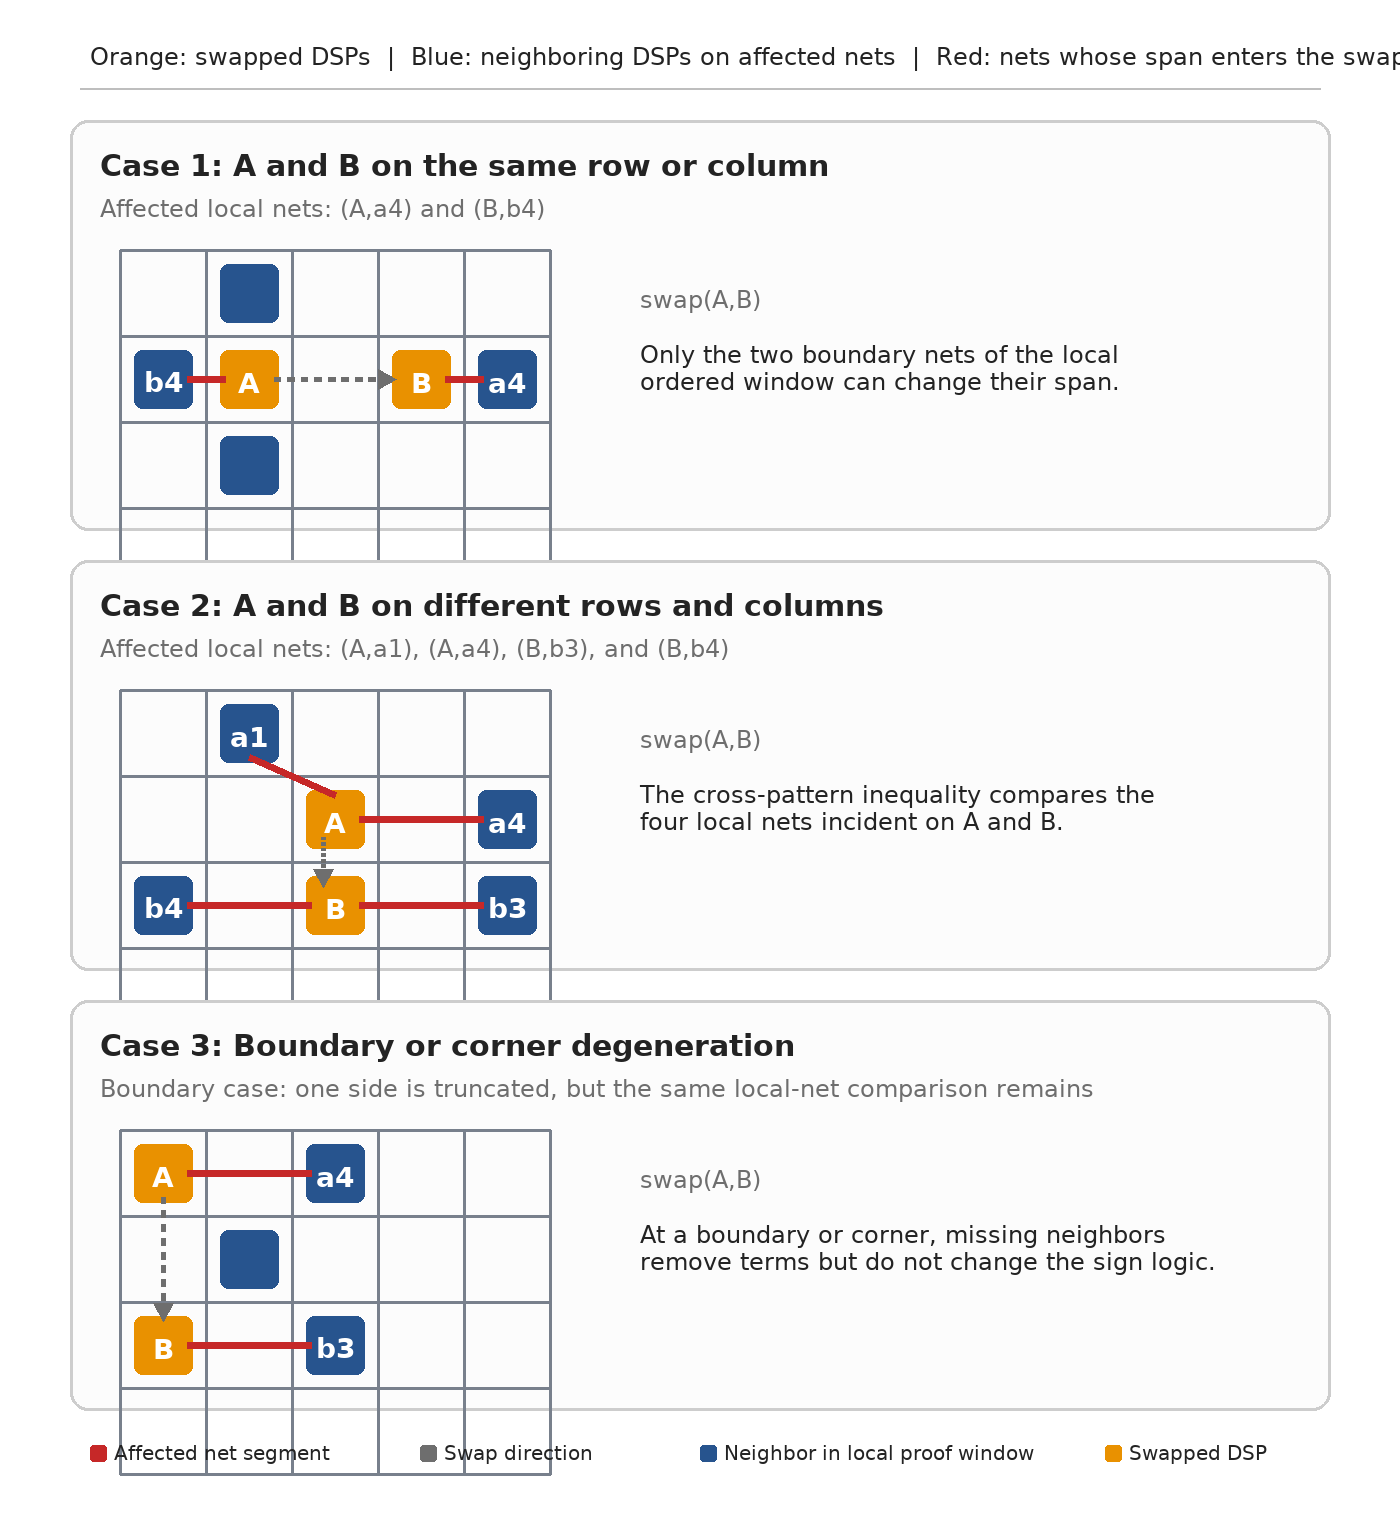
\includegraphics[width=0.98\columnwidth]{assets/oc_cases_precise.png}
\Description{Three local swap configurations used in the OC proof sketch. The first panel shows A and B on the same row or column, with affected local nets to neighboring macros. The second panel shows A and B on different rows and columns, with four affected local nets. The third panel shows a boundary or corner degeneration with truncated neighbors.}
\caption{Local swap patterns and affected nets in the OC proof sketch. The three panels correspond to the same-row or same-column case, the different-row and different-column case, and a boundary or corner degeneration. Red segments denote the local nets whose span enters the swap-local HPWL comparison, while blue blocks mark the neighboring DSPs referenced by the proof.}
\label{fig:oc_cases}
\end{figure}

For each pattern, the incident nets are partitioned into three groups: nets that are forced to become longer after the swap, nets whose contribution is unchanged, and nets that may become shorter. The key observation is that the forced increases always dominate the possible decreases, so the total HPWL change is nonnegative. Figure~\ref{fig:oc_cases} provides an intuitive view of the three local swap patterns. Two algebraic motifs summarize the calculation.

Let $Y(\cdot)$ denote the row or column coordinate used in the corresponding local comparison window. In other words, $Y(a)$, $Y(a_1)$, and related terms denote the ordered coordinate values that appear in the swap-local HPWL calculation for the pattern under discussion.

For the same-row or same-column pattern,
\begin{equation}
\Delta \mathrm{HPWL} = 2\bigl(Y(a4)-Y(b4)\bigr) \ge 0,
\label{eq:swap_same_line}
\end{equation}
where the neighboring terms appear in matched pairs and the swap can only preserve or increase the total span.

For the different-row/different-column pattern,
\begin{equation}
\Delta \mathrm{HPWL}
=
2\bigl(Y(a4)+Y(a1)-Y(b3)-Y(b4)\bigr) \ge 0.
\label{eq:swap_cross}
\end{equation}
This is the core cross-pattern inequality in the slide proof. Boundary and corner cases do not require separate principles; they reduce to the same two algebraic comparisons together with strictly positive contributions from nearby nets that are forced to lengthen after the swap.

Therefore, for any pair of DSP macros and for any swap distance, a two-swap applied to an OC-optimal solution cannot decrease HPWL. Proposition 1 follows.

This is the scientific role of \rsad in the present paper. OC is not introduced here as a heuristic convenience. Rather, it identifies a structured solution space that remains consistent with HPWL optimality in the single-column setting. Only after this justification do we impose OC and use it as the basis of the exact optimization framework below.

\subsection{From OC to an Ordered Objective}

After the above justification, we impose the order-consistency (OC) condition
\begin{equation}
y_{i,j} \le y_{i,j+1}, \qquad y_{i,j} \le y_{i+1,j},
\label{eq:oc}
\end{equation}
which is exactly the monotonicity structure introduced by \rsad.

Under OC, the relative order of every macro pair in a net is fixed. Therefore, each term $|y_{i_a,j_a}-y_{i_b,j_b}|$ in Eq.~(\ref{eq:weighted_hpwl}) has a determined sign and can be rewritten without the absolute value. Summing over all nets yields an ordered linear objective
\begin{equation}
\sum_{i,j} C_{i,j} y_{i,j},
\label{eq:ordered_linear}
\end{equation}
where $C_{i,j}$ aggregates the signed contributions of all incident nets to location $(i,j)$. This is the key algebraic step: once OC fixes pairwise ordering, the \hpwl objective is transformed from an unordered absolute-value objective into an ordered linear objective over placement labels.

\subsection{From Ordered Objective to State DAG}

Eq.~(\ref{eq:ordered_linear}) can be further rewritten into an incremental form indexed by placement order. For each location $(i,j)$, define
\begin{equation}
\phi_{i,j} = d_V \Bigl(
\underbrace{w^V_{i-1,j}}_{\text{up}}
\,+\,
\underbrace{w^H_{i,j-1}}_{\text{left}}
\,-\,
\underbrace{w^V_{i,j}}_{\text{down}}
\,-\,
\underbrace{w^H_{i,j}}_{\text{right}}
\Bigr),
\label{eq:phi}
\end{equation}
with out-of-range terms treated as zero. Here $\phi_{i,j}$ is the local coefficient of location $(i,j)$ in the ordered objective. If order label $\ell+1$ is assigned to location $(i,j)$, the incremental contribution is
\begin{equation}
c_{\ell}(i,j) = (\ell+1)\,\phi_{i,j}.
\label{eq:incremental_cost}
\end{equation}
Thus the total objective can be accumulated one placement step at a time.

We now define the state space. At level $\ell$, a state is
\begin{equation}
a = (a_1,\dots,a_m),
\end{equation}
where $a_i \in \{0,\dots,h\}$ is the number of already placed macros in row $i$, and $\ell=\sum_i a_i$ is the number of already assigned labels. Under OC, the frontier must remain monotone:
\begin{equation}
a_1 \ge a_2 \ge \cdots \ge a_m.
\label{eq:state_monotone}
\end{equation}
The source state is $(0,\dots,0)$ and the sink state is $(h,\dots,h)$.

\begin{figure}[t]
\centering
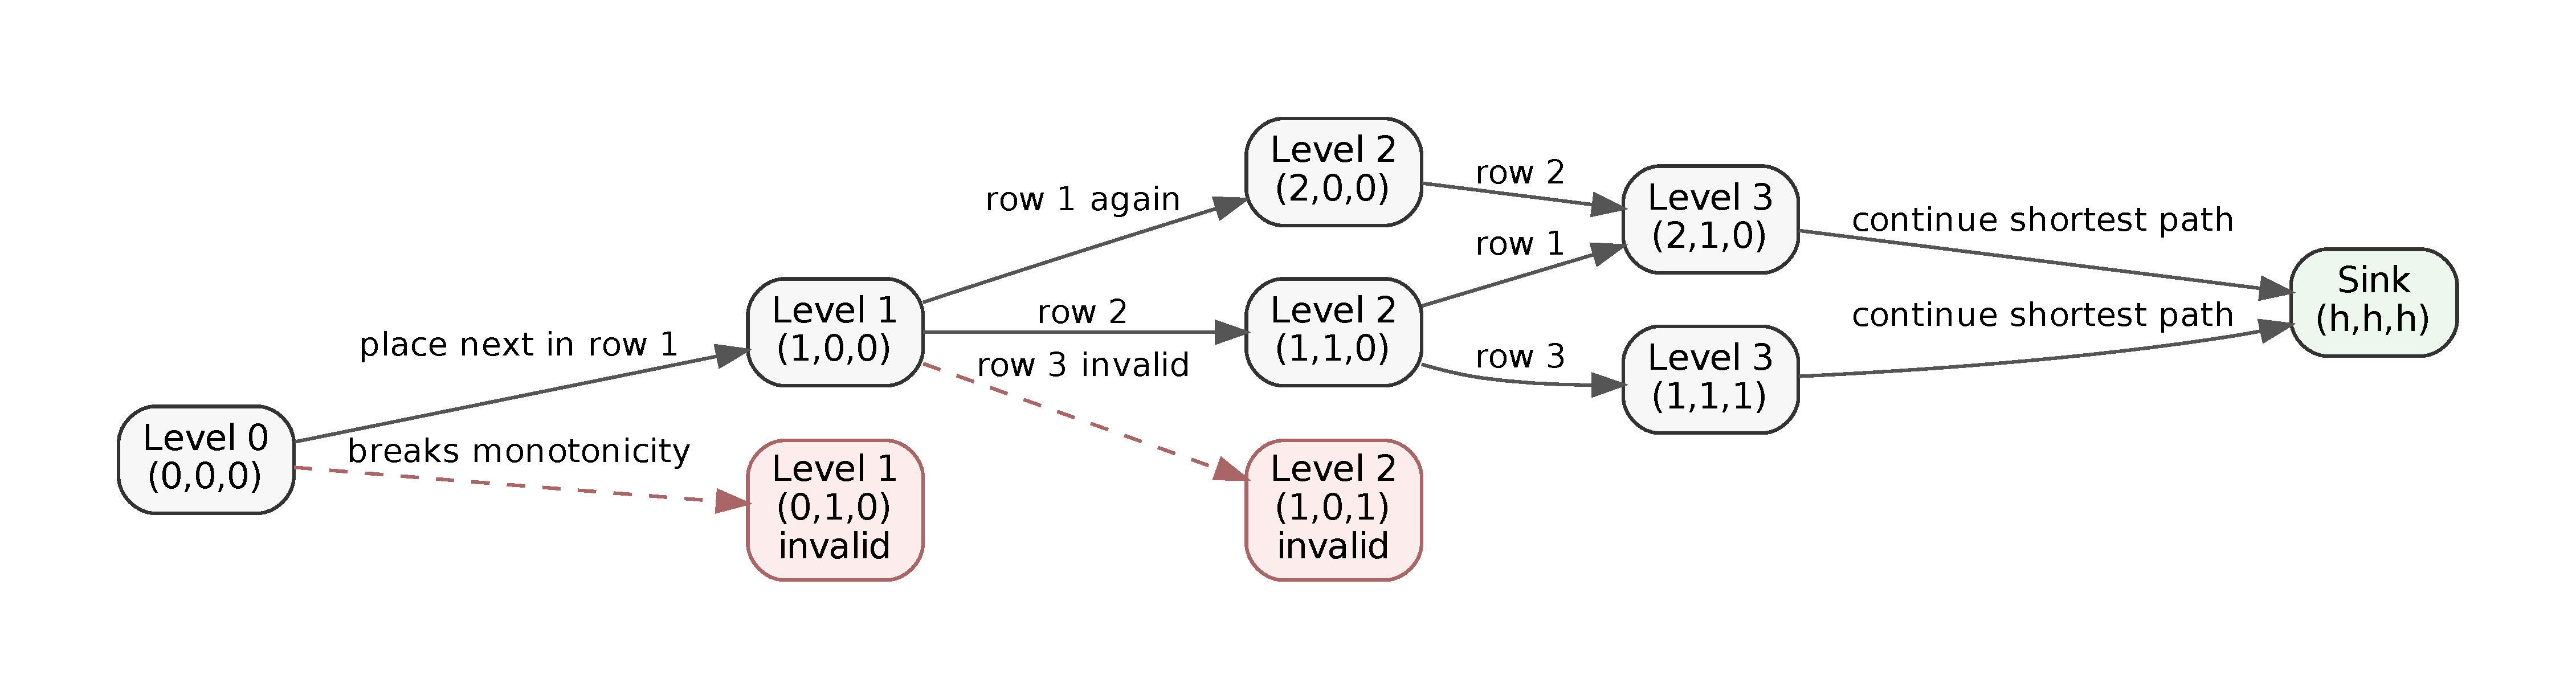
\includegraphics[width=0.95\columnwidth]{assets/state_dag_frontier.pdf}
\Description{A state-DAG illustration in which each node records how many positions have been filled in each row, and each valid edge increments one row count while preserving a monotone frontier.}
\caption{State-DAG view of the OC-constrained strip placement problem. A state records the monotone placement frontier, and each edge places exactly one new macro.}
\label{fig:state_dag}
\end{figure}

An edge in the DAG corresponds to incrementing exactly one row count. If state $a'$ is obtained from $a$ by increasing $a_i$ by one, then the next order label is assigned to location $(i,a_i+1)$. The move is legal only if the frontier remains monotone. Therefore each source-to-sink path corresponds to one feasible OC placement, and the path cost is the sum of all incremental costs. Let $\mathcal{P}(s,t)$ denote the set of all source-to-sink paths in the state DAG. The original optimization is reduced to
\begin{equation}
\min_{P \in \mathcal{P}(s,t)} \sum_{(a,a') \in P} c(a,a'),
\label{eq:dag_shortest_path}
\end{equation}
which is a shortest-path problem on a DAG.

\textbf{Key contribution.}
The main theoretical contribution of this paper is exactly this conversion from optimizing many weighted net HPWL terms to optimizing one shortest path on a state DAG.

\subsection{Dynamic Programming Solver}

Let $f_\ell(a)$ denote the minimum cost of reaching state $a$ after placing the first $\ell$ labels. Since the graph is acyclic, the DP recurrence is
\begin{equation}
f_{\ell+1}(a') = \min_{a \to a'} \bigl(f_\ell(a) + c(a,a')\bigr).
\label{eq:dp}
\end{equation}
The optimal placement is recovered by tracing the minimum-cost source-to-sink path. A forward-backward reconstruction scheme can be used to avoid storing the full DP table.

\subsection{CTR-Based Acceleration}

The exact DP solver is expensive on tall strips. A key acceleration is the central row-sweep (CTR) observation inherited from the \rsad line. When mapping an $m \times h$ array to one DSP column and $m > h > 6$, the middle part of the optimal placement exhibits a row-sweep pattern, called the CTR region in \rsad. What begins as an empirical observation can be converted into an algorithmic reduction.

Instead of solving the full $m \times h$ strip directly, we shrink it to an $h \times h$ core problem, solve that core exactly, and then expand the solution back to the original height. Concretely, the top and bottom bands are preserved from the solved square core, while the middle rows are filled by a row-sweep CTR band. In effect, an $m \times h$ mapping problem is converted into an $h \times h$ problem, and the resulting square solution is split into top and bottom parts with a row-sweep region inserted in the middle. This substantially reduces the computational burden while preserving the structural quality of the placement.

\subsection{Timing-Driven Weight Update}

The exact strip solver is placed inside an outer timing-driven loop. Starting from initial weights, the solver produces a weighted OC placement. That placement is then analyzed to obtain the longest edge, \wns, and \tns under the target $T$.

For each edge $e$, let $L_e$ denote its current geometric length. The slack-like quantity is
\begin{equation}
s_e = T - L_e.
\end{equation}
If all tracked edges satisfy $s_e \ge 0$, the current strip already satisfies the target. Otherwise, the most critical edges receive larger weights.

The weight update borrows the net-weight adaptation style used in DreamPlace 4.0~\cite{dreamplace4}. The solver keeps log-weights and momentum buffers:
\begin{equation}
\Delta \log w_e^{(t+1)} = \alpha\,\Delta \log w_e^{(t)} + \eta \log\bigl(1+c_e^{(t)}\bigr),
\label{eq:dreamplace_style_1}
\end{equation}
\begin{equation}
\log w_e^{(t+1)} = \log w_e^{(t)} + \Delta \log w_e^{(t+1)}.
\label{eq:dreamplace_style_2}
\end{equation}
Here $c_e^{(t)}$ is derived from the current violation magnitude, and only the most critical edges are strengthened in each round.

This creates a clean division of labor:
\begin{itemize}[leftmargin=*,topsep=2pt,itemsep=2pt]
\item the inner DP layer solves the weighted OC strip-placement problem exactly for fixed weights, and
\item the outer loop changes those weights to reduce the longest wires and improve timing.
\end{itemize}

This also explains the empirical tradeoff against \rsad. \rsad is highly effective when the objective is static HPWL minimization under OC. Our method keeps that OC structure and near-optimal HPWL behavior, but additionally drives down the longest wires, which yields better \wns and \fmax at the cost of only a very small HPWL increase.

\subsection{Discussion of Optimality Scope}

The exact optimality claim of this paper applies to the weighted state-DAG subproblem for a fixed set of net weights. The full timing-driven flow remains iterative because weights change between solves. Accordingly, the paper should claim:
\begin{itemize}[leftmargin=*,topsep=2pt,itemsep=2pt]
\item exact shortest-path optimality for the fixed-weight OC subproblem, and
\item empirical timing improvement for the full timing-driven outer loop.
\end{itemize}

\section{Experimental Setup and Results}
\label{sec:exp}

\subsection{Setup}

The current comparison table reports seven benchmarks and five methods. The experiments compare the proposed timing-driven dynamic-programming (DP) flow against Vivado, \rsad, AMFPlace 2.0 + Vivado P\&R, and DSPlace + Vivado P\&R. The target audience should read the first two comparisons differently:
\begin{itemize}[leftmargin=*,topsep=2pt,itemsep=2pt]
\item Vivado is the industrial baseline.
\item \rsad is the direct predecessor and isolates the value of the new timing-driven formulation over the prior OC-based HPWL-oriented deterministic method.
\end{itemize}

This distinction is important. Relative to Vivado, the paper should emphasize that problem-specific systolic-array placement already has large value. Relative to \rsad, the paper should emphasize that the new contribution is not better HPWL minimization alone, but a better timing tradeoff through explicit control of the longest wirelength.

\subsection{Main Results}

The current quantitative outcomes are already sufficient to anchor the paper's central story. Averaged over the seven benchmarks, the proposed flow achieves 249.08\,MHz \fmax, compared with 231.91\,MHz for Vivado and 237.70\,MHz for \rsad. This corresponds to a 7.4\% \fmax gain over Vivado and a 4.8\% gain over \rsad. In terms of wirelength, the proposed flow reduces average \hpwl from 683{,}314 to 519{,}018 relative to Vivado, while remaining very close to \rsad (509{,}232 versus 519{,}018, only +1.9\%).

The timing metrics are consistent with the same story. Compared with Vivado, the proposed flow reduces the magnitude of average worst negative slack (\wns) from 0.71 to 0.39 and the magnitude of average total negative slack (\tns) from 1311.67 to 952.81. Compared with \rsad, it reduces the magnitude of average \wns from 0.61 to 0.39 and the magnitude of average \tns from 1245.90 to 952.81. These numbers suggest two points. First, the timing-driven objective is effective in moving the design toward better timing, which is consistent with the intended longest-wirelength control path. Second, the small \hpwl regression against \rsad indicates that the new method is not simply a wirelength minimizer; it is trading a very small amount of aggregate wirelength for stronger timing quality.

\begin{table}[t]
\caption{Average results over seven benchmarks.}
\label{tab:main}
\centering
\small
\begin{tabular}{lcccc}
\toprule
Method & HPWL & WNS & TNS & \fmax \\
\midrule
Vivado & 683{,}314 & -0.71 & -1311.67 & 231.91 \\
\rsad  & 509{,}232 & -0.61 & -1245.90 & 237.70 \\
AMFPlace2.0 + Vivado P\&R & 927{,}999 & -4.99 & -12837.49 & 117.46 \\
DSPlace + Vivado P\&R & 746{,}915 & -1.67 & -5634.44 & 191.72 \\
Ours   & 519{,}018 & -0.39 & -952.81 & 249.08 \\
\bottomrule
\end{tabular}
\end{table}

\begin{table*}[t]
\caption{Benchmark-wise \hpwl and \fmax comparison for all five methods.}
\label{tab:bench_hpwl_fmax}
\centering
\scriptsize
\resizebox{\textwidth}{!}{%
\begin{tabular}{l|rr|rr|rr|rr|rr}
\toprule
& \multicolumn{2}{c|}{Vivado} & \multicolumn{2}{c|}{\rsad} & \multicolumn{2}{c|}{AMFPlace 2.0 + Vivado P\&R} & \multicolumn{2}{c|}{DSPlace + Vivado P\&R} & \multicolumn{2}{c}{Ours} \\
Case & \hpwl & \fmax & \hpwl & \fmax & \hpwl & \fmax & \hpwl & \fmax & \hpwl & \fmax \\
\midrule
OS24x24\_W8 & 245232 & 263.71 & 177188 & 261.99 & 282005 & 136.91 & 292413 & 241.25 & 177441 & 262.54 \\
OS32x32\_W8 & 494792 & 239.06 & 356790 & 222.52 & 628927 & 121.86 & 543872 & 187.62 & 376203 & 244.92 \\
OS36x32\_W8 & 555410 & 202.51 & 568842 & 246.61 & 908625 & 116.55 & 650782 & 194.67 & 578173 & 247.71 \\
OS40x32\_W8 & 690842 & 230.41 & 448668 & 198.41 & 969454 & 124.35 & 781080 & 180.57 & 475704 & 244.56 \\
OS40x36\_W8 & 774885 & 238.55 & 540131 & 246.79 & 993061 & 116.89 & 880601 & 173.22 & 539512 & 250.50 \\
OS40x40\_W8 & 854961 & 233.26 & 597408 & 245.34 & 1704262 & 104.01 & 982803 & 184.26 & 593826 & 248.45 \\
OS44x40\_W8 & 1167074 & 215.84 & 875596 & 242.25 & 1009659 & 101.68 & 1096855 & 180.44 & 892266 & 244.86 \\
\midrule
AVG & 683314 & 231.91 & 509232 & 237.70 & 927999 & 117.46 & 746915 & 191.72 & 519018 & 249.08 \\
\bottomrule
\end{tabular}
\vspace{-4pt}
}
\end{table*}

\begin{table*}[t]
\caption{Benchmark-wise \wns and \tns comparison for all five methods.}
\label{tab:bench_wns_tns}
\centering
\scriptsize
\resizebox{\textwidth}{!}{%
\begin{tabular}{l|rr|rr|rr|rr|rr}
\toprule
& \multicolumn{2}{c|}{Vivado} & \multicolumn{2}{c|}{\rsad} & \multicolumn{2}{c|}{AMFPlace 2.0 + Vivado P\&R} & \multicolumn{2}{c|}{DSPlace + Vivado P\&R} & \multicolumn{2}{c}{Ours} \\
Case & \wns & \tns & \wns & \tns & \wns & \tns & \wns & \tns & \wns & \tns \\
\midrule
OS24x24\_W8 & -0.29 & -273.47 & -0.32 & -297.27 & -3.70 & -4584.19 & -0.55 & -485.23 & -0.31 & -351.68 \\
OS32x32\_W8 & -0.58 & -1298.78 & -0.89 & -2289.01 & -4.61 & -9662.71 & -1.73 & -4358.38 & -0.48 & -1455.69 \\
OS36x32\_W8 & -1.34 & -1537.04 & -0.46 & -1002.22 & -4.98 & -12272.79 & -1.54 & -4260.06 & -0.44 & -988.01 \\
OS40x32\_W8 & -0.74 & -1564.21 & -1.44 & -2285.96 & -4.44 & -12776.95 & -1.94 & -6675.55 & -0.49 & -1239.85 \\
OS40x36\_W8 & -0.59 & -1442.15 & -0.45 & -1115.90 & -4.96 & -13466.69 & -2.17 & -7940.15 & -0.39 & -1055.06 \\
OS40x40\_W8 & -0.39 & -39.24 & -0.18 & -22.46 & -6.01 & -20995.48 & -1.83 & -6782.90 & -0.13 & -12.35 \\
OS44x40\_W8 & -1.03 & -3026.82 & -0.53 & -1708.49 & -6.24 & -16103.59 & -1.94 & -8938.83 & -0.48 & -1567.06 \\
\midrule
AVG & -0.71 & -1311.67 & -0.61 & -1245.90 & -4.99 & -12837.49 & -1.67 & -5634.44 & -0.39 & -952.81 \\
\bottomrule
\end{tabular}
}
\end{table*}

\subsection{Interpretation}

The paper should interpret these results through the mechanism, not only through the percentages. Tables~\ref{tab:bench_hpwl_fmax} and~\ref{tab:bench_wns_tns} show that the proposed method is the most timing-effective approach among all five compared methods: it delivers the best average \fmax and the best average timing-slack metrics, while keeping \hpwl close to \rsad and substantially better than the three placement-and-route baselines built around generic flows. This is exactly the behavior expected from the method. Explicitly limiting the longest wirelength is a practical path to lowering \wns and improving \fmax. This is why \fmax should remain the first metric in the result discussion, while \hpwl serves as the supporting tradeoff metric. The role of \rsad should also be stated carefully: \rsad remains the stronger \hpwl-oriented predecessor because it exploits the OC structure effectively, and our method wins by adding timing awareness on top of that same structural foundation.

\subsection{Pending Insertions}

The next revision should add:
\begin{itemize}[leftmargin=*,topsep=2pt,itemsep=2pt]
\item one ablation on the timing-driven weight update,
\item one case-study figure showing a representative placement effect, and
\item a short paragraph discussing why \rsad can still be better in pure \hpwl on some cases while losing in \fmax.
\end{itemize}

\section{Conclusion}
\label{sec:conclusion}

This paper presents a timing-driven DSP placement method for systolic arrays on FPGAs. The central contribution is a dynamic-programming formulation that converts the optimization of multiple weighted net \hpwl terms into the shortest-path optimization of a state DAG. This formulation builds on the OC structure introduced by \rsad, clarifies why that structure is valuable for HPWL optimization, and extends it to the weighted timing-driven setting. Experimental results on seven benchmarks show that the resulting flow improves average \fmax over both Vivado and the previous \rsad-based method while keeping \hpwl very close to \rsad. These results support the view that controlling the longest wirelength is an effective path toward lowering \wns and improving timing quality in systolic-array DSP placement without sacrificing the structural advantages of the OC-based formulation.


\bibliographystyle{ACM-Reference-Format}
\begin{thebibliography}{9}

\bibitem{rsad2023}
H. Hu, D. Fang, W. Li, B. Yuan, and J. Hu,
``Systolic Array Placement on FPGAs,''
in \emph{Proc. IEEE/ACM Int. Conf. Computer-Aided Design (ICCAD)}, 2023.

\bibitem{sysmix2024}
D. Fang, H. Hu, W. Li, B. Yuan, and J. Hu,
``SysMix: Mixed-Size Placement for Systolic-Array-Based Hierarchical Designs,''
in \emph{Proc. IEEE/ACM Int. Conf. Computer-Aided Design (ICCAD)}, 2024.

\bibitem{date2021}
Z. Lin, Y. Xie, G. Qian, J. Chen, S. Wang, J. Yu, and Y.-W. Chang,
``Timing-Driven Placement for FPGAs with Heterogeneous Architectures and Clock Constraints,''
in \emph{Proc. Design, Automation and Test in Europe (DATE)}, 2021.

\bibitem{ispd2017}
S. Dhar, M. A. Iyer, S. Adya, L. Singhal, N. Rubanov, and D. Z. Pan,
``An Effective Timing-Driven Detailed Placement Algorithm for FPGAs,''
in \emph{Proc. Int. Symp. Physical Design (ISPD)}, 2017.

\bibitem{ripplefpga2016}
J. Pui, S. Choi, A. Chowdhury, W. Li, S. Tang, D. Z. Pan, Y. Ye, and X. Yang,
``RippleFPGA: A Routability-Driven Placement for Large-Scale Heterogeneous FPGAs,''
in \emph{Proc. IEEE/ACM Int. Conf. Computer-Aided Design (ICCAD)}, 2016.

\bibitem{utplacef2017}
Y. Li, B. Liao, C. Weng, and D. Z. Pan,
``UTPlaceF 3.0: A Parallelization Framework for Modern FPGA Global Placement,''
in \emph{Proc. IEEE/ACM Int. Conf. Computer-Aided Design (ICCAD)}, 2017.

\bibitem{dreamplace4}
P. Liao, D. Guo, Z. Guo, S. Liu, Y. Lin, and B. Yu,
``DREAMPlace 4.0: Timing-Driven Placement With Momentum-Based Net Weighting and Lagrangian-Based Refinement,''
\emph{IEEE Trans. Comput.-Aided Design Integr. Circuits Syst.}, vol. 42, no. 10, pp. 3374--3387, 2023.

\end{thebibliography}


\end{document}
